\documentclass[a4paper]{report}
\usepackage[T1]{fontenc}
\usepackage{amsfonts}
\usepackage{mathbbol}
\usepackage[utf8]{inputenc}
\usepackage[english]{babel}
\usepackage{graphicx}
\usepackage{wrapfig}
\usepackage{float}
\usepackage{lipsum}
\usepackage{fancyvrb}
\usepackage{natbib}


\title{Adaptive Bitrate Streaming: a buffer-based approach } 

\author{Piergiorgio Ladisa
\\
Nicola Sebastianelli}
\date{22/11/2018}


\makeindex

\begin{document}
\maketitle
\tableofcontents
\listoffigures
\newpage

\part*{Buffer-based ABR Algorithm}
These days we are witnessing to the continuous growing demand of streamed content in network: anyone asks anywhere and in any-moment for contents to servers from their mobile devices. Hence, since the percentage of contents in the network is becoming everyday bigger, CDNs and ISPs are called to respond to this demand.
The paradigm of the multimedia systems and for CDN is mainly the so-called Quality of Experience (QoE). This is very different from the paradigm on which Internet was designed, i.e. Quality of Service (QoS) and Best Effort, in fact the quality of experience is really subjective and very difficult to measure. Nevertheless, different protocols and strategies have been proposed in order to met the demand of users of streaming of contents. 
Firstly, different strategies of streaming exists:
\begin{itemize}
\item all-in-once, i.e. the content is entirely sent to the user. This approach is enforced by the server and the encoding rate is unintentional, since the client's buffer is filled up, in the same way in which the TCP buffer is filled up; since TCP performs the flow control, the client with this approach read at the encoding rate;
\item throttling, i.e. the rate is adapted to the user with two possible approach:
\begin{itemize}
\item on-off-S, in which the connection is maintained persistently;
\item on-off-M, in which the connection is not maintained persistently
\end{itemize}
These two approaches are caused by the client application, that periodically stops reading from the TCP socket. In a general case of  pseudo-streaming, the video is buffered until the buffer is enough full and, once reached the steady state, the controller starts doing an on-off step, downloading the block size of the video.
\end{itemize}
In this context, the mainly adopted protocol is HTTP Adaptive Streaming protocol (HAS). Here the idea is to make the requested bitrate of the video fit with the varying network resources, ensuring the best possible quality of experience for the user, based on the current situation of the network.
This adaptation is usually done on client-side. Here the content is divided in chunks and available in different qualities. So HAS allows to encode each segment in different quality referring to the current bandwidth and so the stream is splitted into a sequence of segments, instead of downloading one entire large file (as in the all-in-once approach). The policies of HAS are:
\begin{itemize}
\item Rate-based, that select the highest possible video representation referring to the measured speed from the previous received chunk;
\item Buffer-based, that uses different thresholds for the buffer in a way in which the more the buffer is filled, the more quality of the video is. Thus, with this approach, the quality can switch step-by-steo at each new request of a video segment: it is impossible to jump from the lowest to the highest quality just in one step;
\item Buffer and Rate based. This is an hybrid approach, i.e. is based on the rate-based approach basically, but the previous chunk download speed is weighted using a factor that depends on the amount of the saturation of the buffer: if the buffer is depleting the previous chunk, the download speed will be considered to be less than the measured one and hence a lower quality is selected. 
\end{itemize}

\chapter{A buffer-based approach to rate adaptation}
When the client want to access to a video-content for streaming, it chooses which the video rate to stream by monitoring network conditions and estimating the available network capacity. This process is referred to as \textit{adaptive bit rate selection} or \textit{ABR}.
ABR algorithms try to balance two opposite goals. The first goal is  to maximize the video quality choosing as video rate the highest supportable by the network. The second goal is to minimize re-buffering events, which cause the video to halt if the client?s playback buffer goes empty. Data is requested in chunks and the buffer drains at 1 unit/second. So if the video-rate $R(t)$ is greater than the system capacity $C(t)$, new data is added at $C(T)/R(T)<1$, depleting the buffer.
\begin{figure}[H]
  \begin{center}
    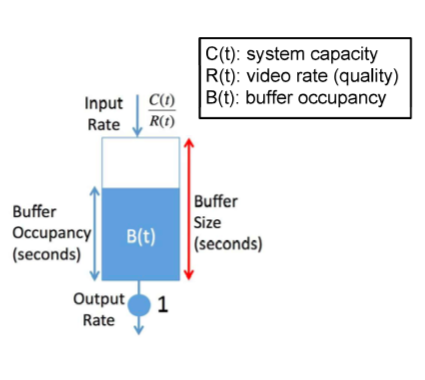
\includegraphics[width=0.5\textwidth]{buffer}
  \end{center}
  \caption{Relationship between system capacity and video rate in video playback buffer ~\citep{Huang:2014:BAR:2740070.2626296} }\label{buffer}
\end{figure}

In order to maximize video quality, a service could just stream at the maximum video rate $R_{max}$ all the time, but this would risk extensive re-buffering. On the other hand, to minimize rebuffering, the service could just stream at the minimum video rate $Rmin$ all the time but this extreme would lead to low video quality. Hence, the design goal of an ABR algorithm is to simultaneously obtain high performance on both metrics in order to give users a good quality of experience.
Firstly, the client measures how fast chunks arrive to estimate capacity, let us say $C\textit{(}t\textit{)}$. The estimate enriched with knowledge of the buffer occupancy, which is represented with an  adjustment factor  $F\textit{(}B\textit{(}t\textit{)}\textit{)}$, i.e. a function of the playback buffer occupancy. So, the selected video rate is $R\textit{(}t\textit{)} = F(B\textit{(}t\textit{)})C\textit{(}t\textit{)}$; different designs use different adjustment functions $F\textit{(}.\textit{)}$.
When the buffer contains many chunks, $R(t)$ can safely deviate from $C(t)$ without triggering a rebuffer. The client can aggressively try to maximize the video quality by picking $R(t) = C(t)$. But when the buffer is low, the client should be more conservative.

We say that an ABR algorithm is \textit{buffer-based} if it picks the video rate as a function of the current buffer occupancy $B(t)$.
The region between:
\begin{itemize}
\item $[0, B_{max}]$ on the buffer-axis;
\item $[R_{min}, R_{max}]$ on the rate-axis;
\end{itemize}
defines the feasible region. So, any curve $f(B)$ on the plane within the feasible region defines a \textit{rate map}, i.e. a function that produces a video rate between $R_{min}$ and $R_{max}$ given the current buffer occupancy.
Let us assume that:
\begin{itemize}
\item the chunk-size is infinitesimal;
\item video rates within $[R_{min}, R_{max}]$ are continuous;
\item videos are encoded at a constant bitrate;
\item videos are infinitely long;
\end{itemize}
Thus, as long as $C(t) \geq R_{min}$ and $f(B)$ tends to $R_{min}$ when $B$ tends to $0$, there will not be unnecessary rebuffering events. So, as long as $f(B)$ increases to $R_{max}$, the average video rate will match the average capacity when it is true that $R_{min}<C(t)<R_{max}$.

\section{BBA0-Algorithm}
The rate map implemented by the BBA0 algorithm is the following:

\begin{figure}[H]
  \begin{center}
    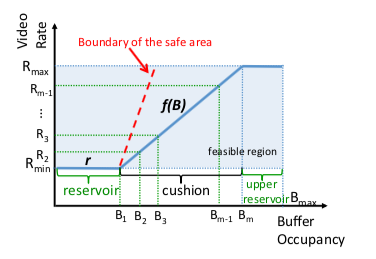
\includegraphics[width=0.7\textwidth]{ratemapBBA0}
  \end{center}
  \caption{Rate map of the BBA0 algorithm ~\citep{Huang:2014:BAR:2740070.2626296} }\label{ratemapBBA0}
\end{figure}

This algorithm add reservoir $r$ to pad for finite chunk sizes and some $C(t)$ variation. So, while filling reservoir, it request $R_{min}$ and must have $r$ greater or equal to the minimum chunk size. In addition, an upper reservoir is added to reach $R_{max}$ before the buffer B is full and above the "safe area" is where the buffer will not deplete into $r$ if $C(t)$ suddenly drops, but does not reach values lower than $R_{min}$.

\subsection{BBA0 Algorithm}
The algorithm presented in ~\citep{Huang:2014:BAR:2740070.2626296}, in pseudo-code, is the following:

\textbf{Input}: 
\begin{itemize}
\item Rate$_{prev}$: previously used video rate;

\item Buf$_{now}$: current buffer occupancy;

\item r: size of reservoir;

\item cu: size of cushion.

\end{itemize}

\textbf{Output}: Rate$_{next}$: next video rate.

\begin{Verbatim}
if Rate_prev = R_max then
	Rate+ = R_max
else
	Rate+ = min{Ri : Ri > Rate_prev}

if Rate_prev = R_min then
	Rate- = R_min
else
	Rate- = max{Ri : Ri < Rate_prev}

if Buf_now <= r then
	Rate_next = R_min

else if Buf_now >= (r + cu) then
	Rate_next = R_max

else if f(Buf_now) >= Rate+ then
	Rate_next = max{Ri : Ri < f(Buf_now)};

else if f(Buf_now) <= Rate- then
	Rate_next = min{Ri : Ri > f(Buf_now)};

else
	Rate_next = Rate_prev;

return Rate_next;
	
	
\end{Verbatim}

This constitute a buffer-based algorithm to the rate adaptation in playing contents from the client.

\subsection{Implementation of BBA0 Algorithm}
The implementation that we have done of the BBA0 algorithm is written in Python and is presented below.

Since the BBA0 Algorithm regards the algorithm for the controller in the player, what we have implemented is a controller used by the player defined in the script \textit{play.py}.

Firstly, we have defined the class BBA0Controller, in order to be imported by the player and executed through the specification of the use of this controller. So the definition of the class is the following:
\begin{Verbatim}

class BBA0Controller(BaseController):

    def __init__(self):
        super(BBA0Controller, self).__init__()

    def __repr__(self):
        return '<BBA0Controller-%d>' % id(self)
\end{Verbatim}


The code below specifies the rate-map function $f(B)$, that is the line passing from the points $(reservoir, R_{min})$ and $(reservoir+cushion, R_{max})$. Hence the equation for the line is the following:

\[
f(B) = B *(\frac{(R_{max} - R_{min})}{cushion} + (R_{min} - \frac{reservoir}{cushion}) * (R_{max} - R_{min})
\]

so, the declaration of the function member of the class requires as input the object itself (i.e., \textit{self}), the current value of the buffer (i.e., \textit{B\_now}), the value for the \textit{reservoir}, the \textit{cushion} and the maximum and minimum values of the rate (i.e., respectively \textit{R\_max} and \textit{R\_min}).

\begin{Verbatim}
    def f(self, B_now, reservoir, cushion, R_max, R_min):
        # The function f corresponds to the line equation between the 
        # points (r,R_min) and (r+cu,R_max) when the value of Buf_now 
        # is bounded by r and r+cu
        return B_now * ((R_max - R_min) / cushion) + 
        		(R_min - ((reservoir / cushion) * (R_max - R_min)))
\end{Verbatim}

The aim of the functions \textit{minR(constraint)} and \textit{maxR(constraint)} is to find the smaller and bigger rate between the available ones that respect a given constraint. In order to compute them, in the \textit{maxR(constraint)} function all the rates that are smaller than the constraint are inserted in the array results and then the bigger of them is selected, in other hand in the \textit{minR(constraint)} function all the rates that are bigger than the constraint are inserted in the array results and then the smaller of them is selected.

\begin{Verbatim}
    def maxR(self, constraint):
        Rates = self.feedback['rates']
        results = []
        for i in Rates:
            if (i < constraint):
                results.append(i)
        return max(results)

    def minR(self, constraint):
        Rates = self.feedback['rates']
        results = []
        for i in Rates:
            if (i > constraint):
                results.append(i)
        return min(results)
\end{Verbatim}

The method member of the class defined below is the actual implementation of the BBA0 algorithm. In order to reproduce the behavior depicted in Figure ~\ref{ratemapBBA0}, the percentages for the
\begin{itemize}
\item \textit{reservoir} is setted at $15\%$;
\item \textit{cushion} is setted at $65\%$;
\item \textit{upper-reservoir} is setted at $20\%$;
\end{itemize}
In addition, the values of R\_max, R\_min, R\_curr and B\_now are taken from the \textit{Base Controller}.
\begin{Verbatim}
    def calcControlAction(self):

        # Retrive current iteration variables
        percentage_reservoir = 0.15
        percentage_cushion = 0.65
        percentage_upper_reservoir = 0.20
        reservoir = self.feedback['max_buffer_time'] * percentage_reservoir
        cushion = self.feedback['max_buffer_time'] * percentage_cushion
        R_max = self.feedback['max_rate']
        R_min = self.feedback['min_rate']
        R_curr = self.feedback['cur_rate']
        B_now = self.feedback['queued_time']
\end{Verbatim}

In this part begin the actual implementation of the BBA0 algorithm, in the same way as it is explained by the pseudo-code in the previous section.

Hence if the current value of the rate during the streaming of the content is equal to the maximum value of the rate, the upper-bound of the rate (i.e., R\_plus) is setted to the maximum value of the rate; otherwise it is setted to the minimum value computed with the function \textit{minR}.
The same logic is adopted to compute the lower-bound of the rate (i.e., R\_minus).
\begin{Verbatim}
        # Compute upperbound
        if R_curr == R_max:
            R_plus = R_max
        else:
            R_plus = self.minR(R_curr)

        # Compute lowerbound
        if R_curr == R_min:
            R_minus = R_min
        else:
            R_minus = self.maxR(R_curr)
\end{Verbatim}

In the following, the goal is to compute the next value of the rate, depending in which region the current value of the buffer lies and we can have four cases :
\begin{enumerate}
\item the current value of the buffer is in the ''lower''-reservoir area: in this case the next value for the rate will be equal to the lower-bound of the rate;

\item the current value of the buffer is in the ''upper''-reservoir area: in this case the next value for the rate will be equal to the upper-bound of the rate;

\item the current value of the buffer is in the cushion area: in this case the rate-map function is applied and:
\begin{itemize}
\item if $f(B) \geq R_{plus}$ then the next value of the rate is calculated as the maximum value of the rate computed with the \textit{maxR} function;
\item otherwise, if $f(B) \leq R_{minus}$ then the next value of the rate is calculated as the minimum value of the rate computed with the \textit{minR} function;
\end{itemize}

\item if none of the previous option is true, then the next value of the rate will be equal to the current one.
\end{enumerate}

\begin{Verbatim}
        # Compute new rate based in current buffer region

        # Buffer in reservoir area
        if B_now <= reservoir:
            Rate_next = R_min

        # Buffer in upper reservoir area
        elif B_now >= reservoir + cushion:
            Rate_next = R_max

        # Buffer in cushion area
        elif self.f(B_now, reservoir, cushion, R_max, R_min) >= R_plus:
            Rate_next = self.maxR(self.f(B_now, reservoir, cushion, R_max, R_min))
        elif self.f(B_now, reservoir, cushion, R_max, R_min) <= R_minus:
            Rate_next = self.minR(self.f(B_now, reservoir, cushion, R_max, R_min))
        
        else:
            Rate_next = R_curr

        return Rate_next

\end{Verbatim}

\subsection{Experiment setup}
As explained in ~\citep{RamonAparicio}, two VMs are used: one that act as server and one as client. The client machine uses the \texttt{192.168.1.1/24} address, while the server machine uses the \texttt{192.168.1.254/24} address.

So, the client play the content using the DASH protocol and a video is hosted on the server. In order to play the video we use the TAPAS player, that act as a DASH player, which generates the HTTP requests for the chunks of the video in different quality, depending on the adaptation algorithm adopted. In our case, the adaptation algorithm, or \textit{controller}, is the BBA0 controller. So, to client-side, from the directory \texttt{~/tapas-master} we execute the command:

\begin{Verbatim}
DEBUG=2 python play.py -m nodec -a BBA0 
	-u http://192.168.1.254/car-20120827-manifest.mpd
\end{Verbatim} 

and the log files of the playing are saved as log files in the client directory \texttt{$\sim$\slash tapas-master\slash log\slash BBA0\slash}.
From these log files we will plot them using the script \texttt{plot\_metrics.sh} located in the directory \texttt{$\sim$\slash Documents\slash scripts}.
Notice that, since the two VMs are not connected by a real network but via virtualization , the values of the bandwidth estimated by the client are simulated as  realistic network bandwidth values using the script called \texttt{bw\_evol.sh} in the folder \texttt{$\sim$\slash Documents\slash scripts}.

Observe that the script \textit{play.py} has been properly modified, in order to include the BBA0 controller.
In addition, the script \textit{plot\_metrics.sh} has been modified in order to automatically oper the most recent file in the folder \texttt{$\sim$\slash tapas-master\slash logs\slash BBA0}, if no file are specified when the script is executed. This is done by adding the following code in the script:

\begin{Verbatim}
if [ ! -z $1 ]
then
log_filename="../../tapas-master/logs/BBA0/$1"
else
log_filename="../../tapas-master/logs/BBA0/$(ls ../../
		tapas-master/logs/BBA0  -Art | tail -n 1)"
fi
echo "Opening: $log_filename"
\end{Verbatim}


\subsection{Results and Conclusion}

We have played the experiments both with the Conventional Controller and the BBA0 Controller, in order to compare the two controllers and spot the difference and also the improvement realized used a buffer-based approach to rate adaptation.
In order to get a valid result and a fair comparison, we have played the same video and using the same environment, described in the previous section

Using the Conventional Controller, the plot of the log file is the following:

\begin{figure}[H]
  \begin{center}
    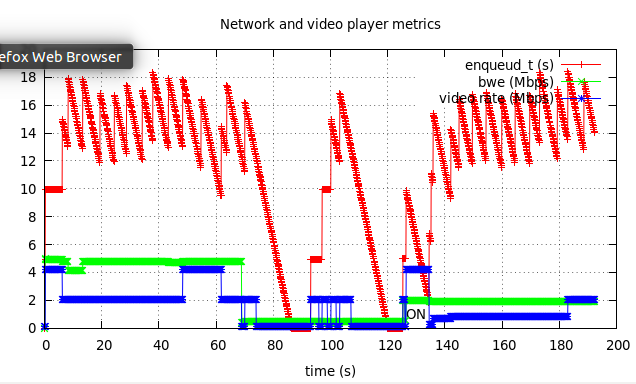
\includegraphics[width=0.7\textwidth]{conventionalcontroller}
  \end{center}
  \caption{Plot of log-file using the Conventional Controller}\label{resten}
\end{figure}

In addition, this controller offers an \textit{average video-rate} of $1.6235484897 Mbps$ and a \textit{total paused-time} of $26.676 s$.


Using the BBA0, the plot of the log file is the following:

\begin{figure}[H]
  \begin{center}
    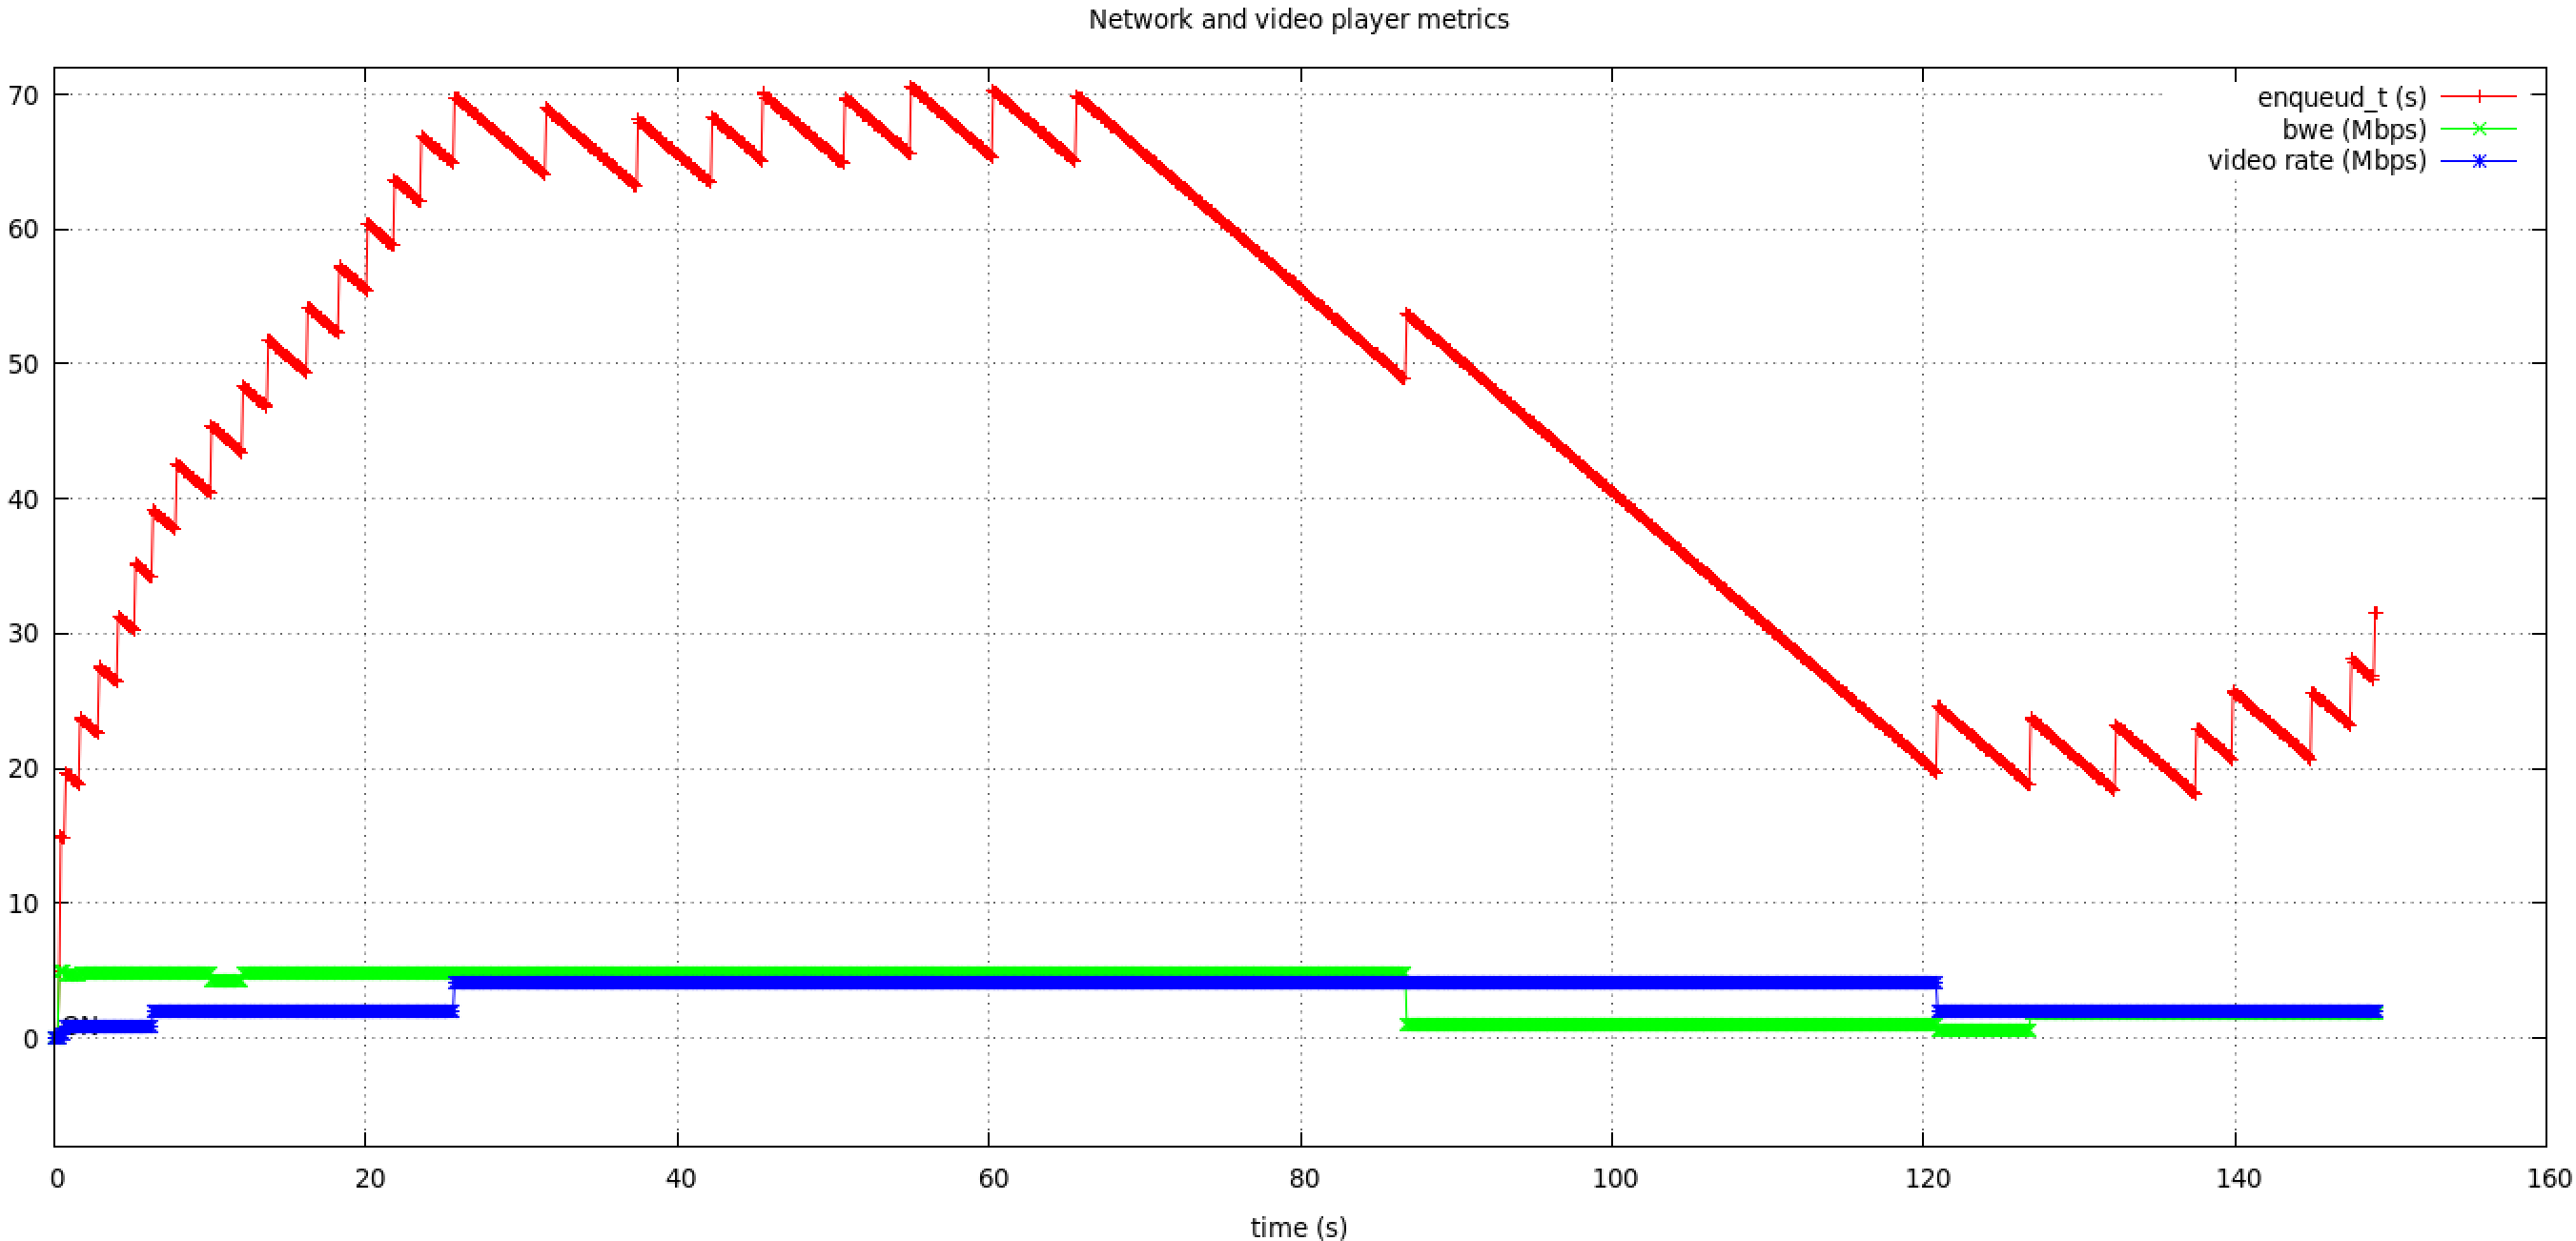
\includegraphics[width=0.7\textwidth]{res_ten_cushion_seventyfive}
  \end{center}
  \caption{Plot of log-file using a reservoir at $10\%$, an upper reservoir at $15\%$ and a cushion at $75\%$}\label{resten}
\end{figure}

\begin{figure}[H]
  \begin{center}
    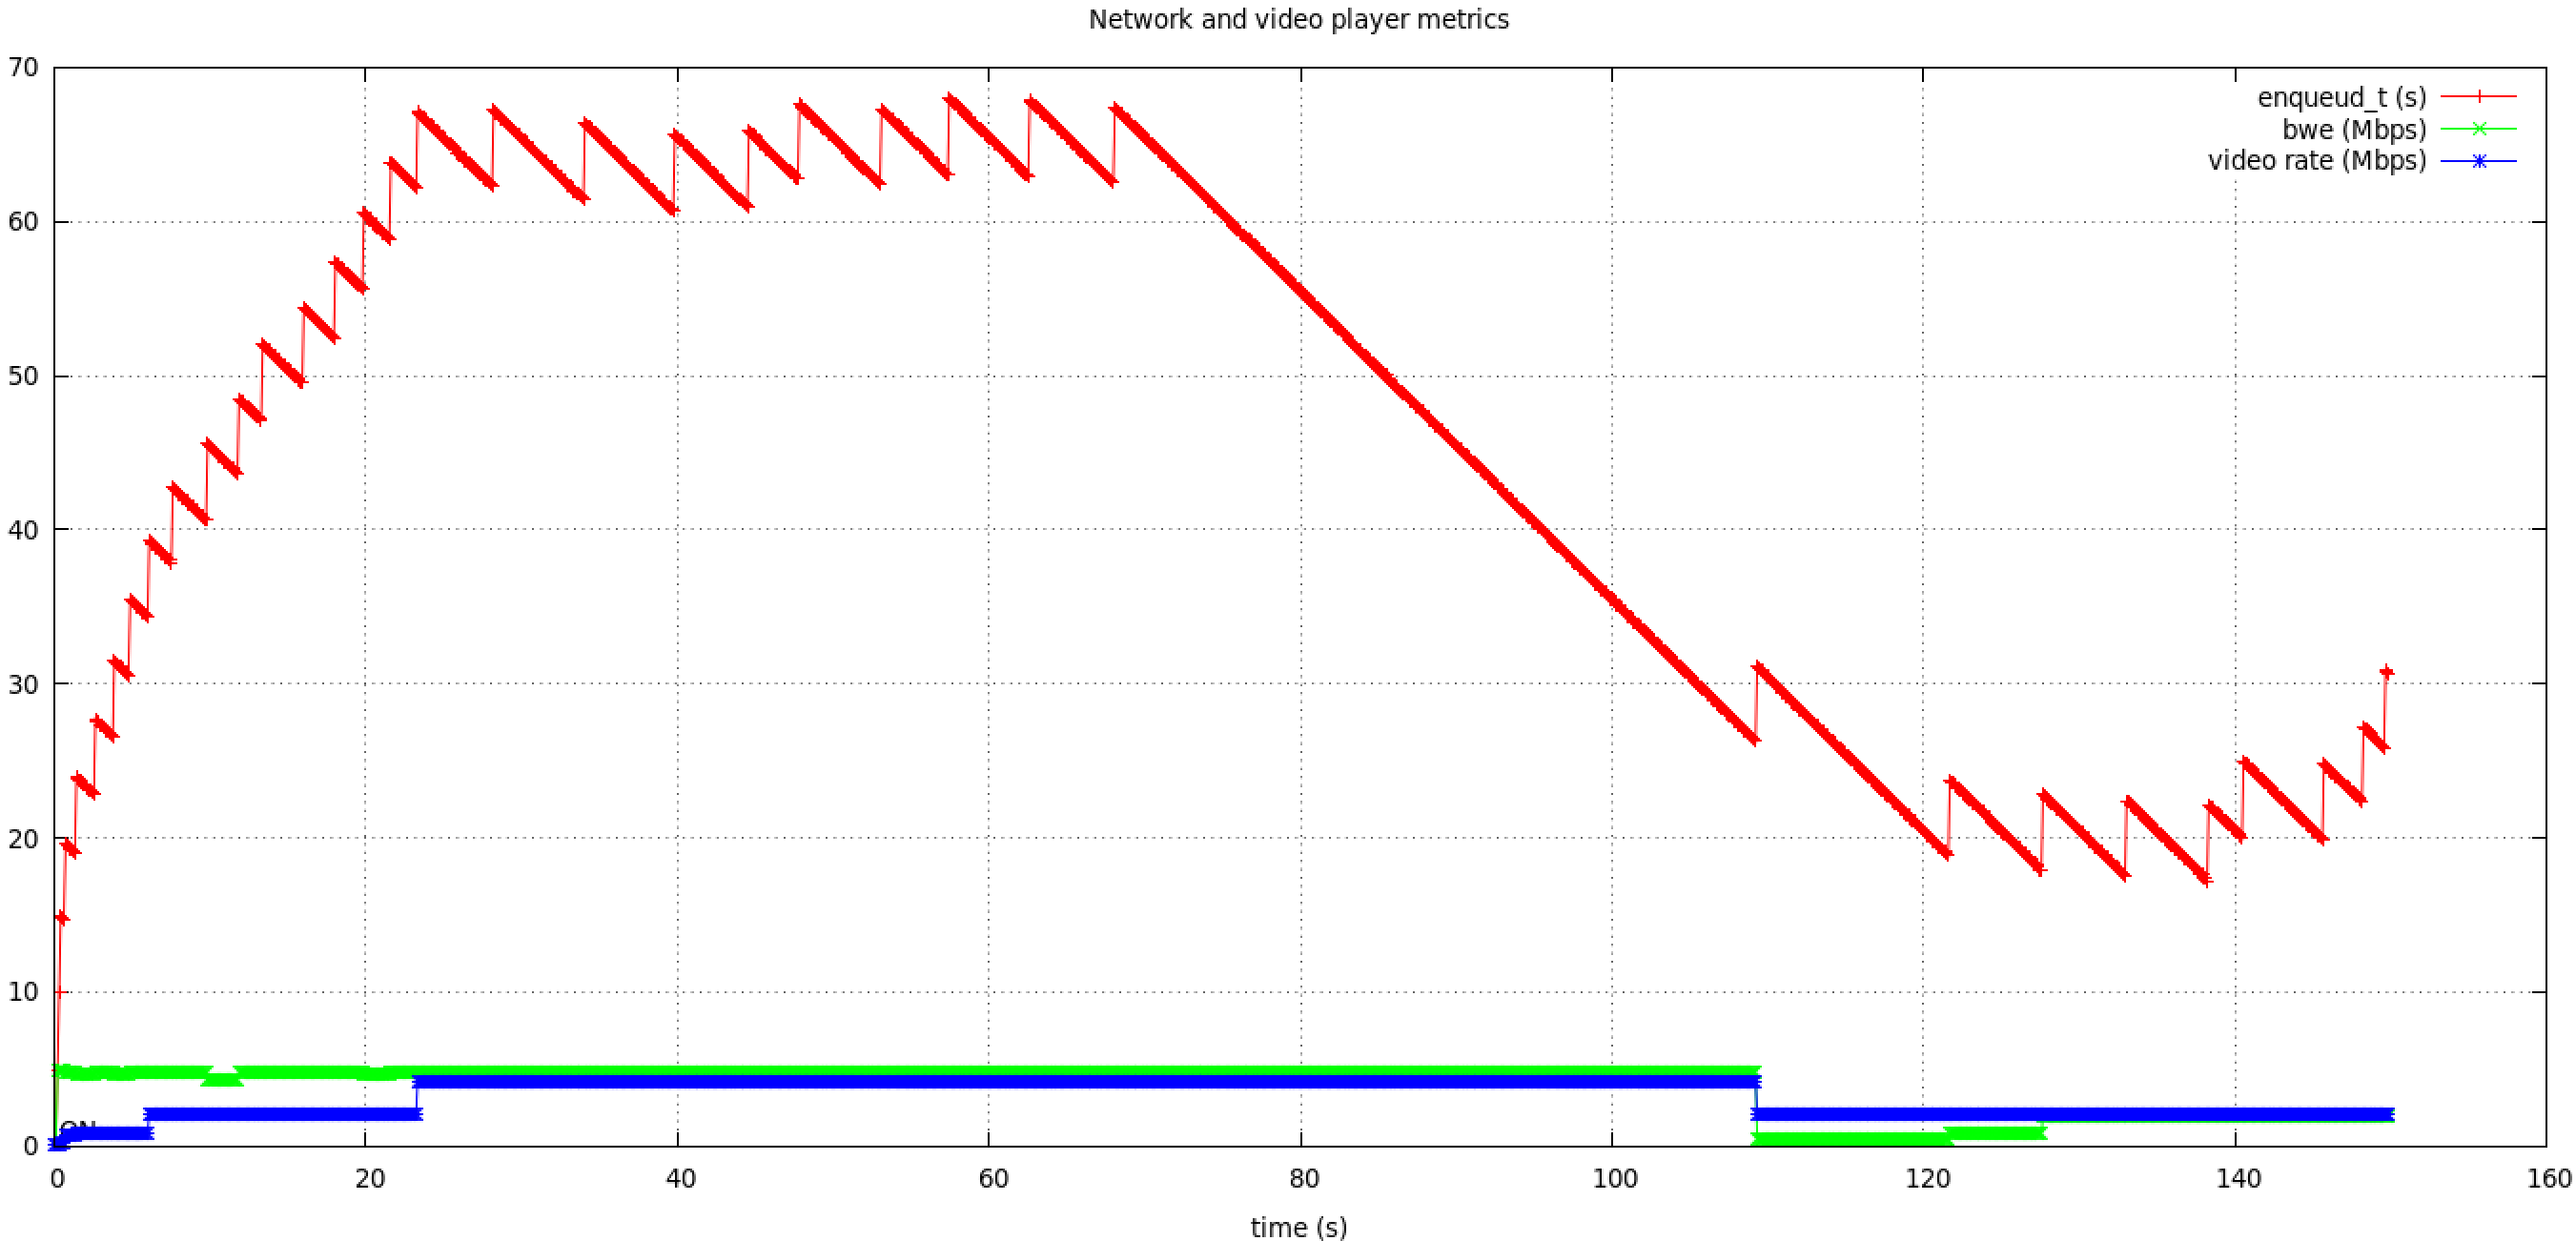
\includegraphics[width=0.7\textwidth]{res_fifteen_cushion_sixtyfive}
  \end{center}
  \caption{Plot of log-file using a reservoir at $15\%$, an upper reservoir at $20\%$ and a cushion at $65\%$}\label{resfifteen}
\end{figure}

With this controller , the \textit{average video-rate} is $3.1608442136 Mbps$, while the \textit{total paused-time} is equal to $0.857 s$

As we can see, with the BBA0 Controller we get a better, so an higher, average video-rate  and a smaller total paused-time: this means that we spend less time, during the streaming, for the buffering and in addition we get a better video-rate, hence a better quality of video-chunks. So the general QoE has improved.

\section{BBA2-Algorithm}
As a further improvement of BBA0-Algorithm, we have implemented a modified version of the BBA2-Algorithm but, since the original BBA2, as explained in ~\cite{Huang:2014:BAR:2740070.2626296}, applies an "aggressive" approach during the start-up phase, then uses the BBA1~\cite{Huang:2014:BAR:2740070.2626296}, instead of using BBA1  we use again BBA0. The reason of that is that BBA1 reasons on the chunk size instead of the rates (compared to BBA0), but in our environment we don't have different chunk size, so we cannot test it. That is why we choosed to switch on BBA0 instead on BBA1 after the start-up phase ends.

During the start-up phase, the playback buffer is empty and it does not have useful information that allow us to choose a video rate. But as we can see from the plot of BBA0 execution, the buffer start with low video rate and, step-by-step, increase until a certain value, than decreases. So, the idea behind BBA2 is the fact during the start-up is possible to improve the video rate, entering in the risky area, i.e. the area above the reservoir and $f(B)$. Hence, BBA2 Algorithm behave more aggressively during the start-up phase, involving a capacity estimation in order to fill the buffer as much as possible, allowing to have an higher video rate than what the rate-map suggests.
Two equivalent models of the streaming playback buffer can be represented as following:

\begin{figure}[H]
  \begin{center}
    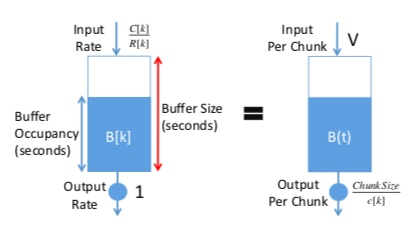
\includegraphics[width=0.7\textwidth]{modelplaybackbuffer.png}
  \end{center}
  \caption{Equivalent models of the streaming playback buffer ~\cite{Huang:2014:BAR:2740070.2626296}}\label{playback}
\end{figure}

From this model we can deduce that the delta of the buffer can be expressed as:

\[
\Delta B = V - (\frac{ChunkSize}{c[k]})
\]

where $V$ is the instantaneous video rate, while the ratio $ChunkSize/c[k]$ represents the system capacity.
Let us assume that the current video rate is $R_i$, in order to safely step up a rate, $c[k]$ needs to be at least equal to $R_{i+1}$ to avoid rebuffers. From this assumption implies that:

\[
\Delta B \geq V - \frac{ChunkSize}{R_{i+1}}
\]

Since videos are encoded in Variable BitRate (VBR), the instantaneous video rate can be higher than the nominal rate. So, indicating with $e$ the \textit{max-to-average} ratio in a VBR stream, the value $eR_{i+1}$ represents the maximum instantaneous video rate in $R_{i+1}$. So, considering a VBR and an empty buffer, it is required that:

\[
\Delta B \geq V - \frac{ChunkSize}{eR_{i+1}}
\]

in order to step up safely from $R_{i}$ to $R_{i+1}$.
In our case the max-to-average ratio $e$ is computed looking at the different segment sizes located in the folder \texttt{\~/Documents/scripts/segments\_quality\#} (where \# is replaced with 0, 1, 2, 3, 4 and 5). Hence, computing the average of the sizes of files in these directory and dividing the maximum size by this average, we get as value of $e \sim 1.69$. In addition $R_{i} / R_{i+1} \sim 2$, so $\Delta B $ needs to be larger than $1 - \frac{0.5}{1.69*2}$. If this condition is true, and so we are in the startup phase, the value picked for the $R_{next}$ is the upper-bound of the rate, i.e. $R^+$. 

\subsection{Implementation of BBA2 Algorithm}

Basing on what we said in the previous section, the implementation of this is presented in the following. 
The code is similar to the BBA0, but what we have added is the definition of $\Delta B$  inside the \textit{calcControlAction()}:

\begin{Verbatim}
delta_B = self.feedback['fragment_duration'] - (self.feedback['last_fragment_size'] / self.feedback['bwe'])
\end{Verbatim}

In fact the istantaneous video rate V is the member of the object \textit{BaseController} named \textit{fragment\_duration}. The \textit{ChunkSize} is the \textit{last\_fragment\_size}, while the capacity for the k-th chunk is represented by the variable \textit{bwe}.

So if the condition for the $\Delta B$ is true, the value for the $R_{next}$ will be $R^+$:

\begin{Verbatim}
if delta_B > (1- 0.5/(1.69*2)) * self.feedback['fragment_duration']:
	    Rate_next = R_plus
\end{Verbatim}

\subsection{Experiment setup}

The experiment setup is the same as for the BBA0 algorithm, in order to make a fair comparison between the two algorithm.

\subsection{Results and Conclusion}

In order to compare the implementation of the (modified) BBA2 algorithm and spot the difference or see if improvements are achieved, we have used the same values for the cushion and reservoir as previously.
In order to get a valid result and a fair comparison, we have played the same video and using the same environment, described in the previous section

Using the (modified) BBA2 algorithm, the plot of the log file is the following:

\begin{figure}[H]
  \begin{center}
    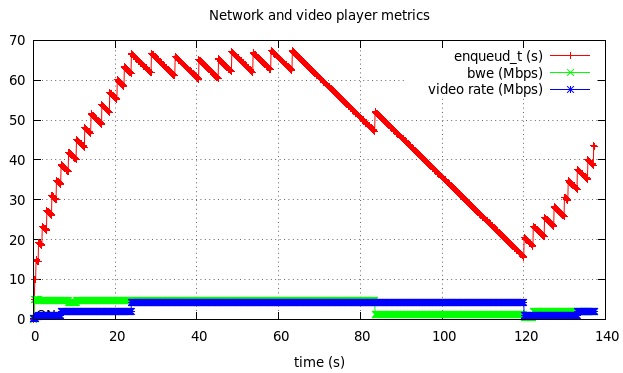
\includegraphics[width=0.7\textwidth]{bba2plot}
  \end{center}
  \caption{Plot of log-file using the BBA2 Controller}\label{resten}
\end{figure}

With this controller , the \textit{average video-rate} is $3.3776721068 Mbps$, while the \textit{total paused-time} is equal to $0.941 s$.
As we can see, we have achieved a better result for the average video rate, compared to the Conventional Controller and the BBA0 Controller: from this implies a better quality for the video. Compared to the BBA0, in addition, we have a worse value for the total-paused time, even if the difference is not so much: in fact we will spend just the $7.2\%$ of time in buffering more than the BBA0.
But from a user perspective, this loss is negligible, since is not so much, but with this improvement is possible to get a better quality for the streaming.


%------- BIBLIOGRAPHY -----------
\bibliography{bibliography}
\bibliographystyle{plain}

\end{document}

